ホームページの閲覧は常にURLの訪問で行われます。ではURLとは一体どういうものなのでしょうか?

URL(Uniform Resource Locator)は"統一資源位置指定子"の英語の短縮です。ネットワーク上のリソースを表現しています。基本的なシンタックスは以下のとおりです。

\begin{lstlisting}[numbers=none]
scheme://host[:port#]/path/.../[?query-string][#anchor]
scheme         低レイヤーで使用されるプロトコルを指定します。
              (例えば:http, https, ftp)
host           HTTPサーバのIPアドレスまたはドメイン
port#          HTTPサーバのデフォルトのポート番号は80です。
               この場合ポート番号は省略することができます。
               もし別のポートを使用する場合は指定しなければなりません。
               例えば http://www.cnblogs.com:8080/
path           リソースまでのパス
query-string   httpサーバへ送るデータ
anchor         アンカー
\end{lstlisting}


DNS(Domain Name System)は"ドメインシステム"の英文の省略です。これは組織の木構造の計算機とネットワークサービスの命名システムです。これはTCP/IPネットワークで使用されます。ホスト名またはドメインを実際のIPアドレスに変換する作業を行う役目を担っています。DNSはこのような翻訳家です。この基本的な動作原理は下の図に示しているとおりです。


\begin{figure}[H]
  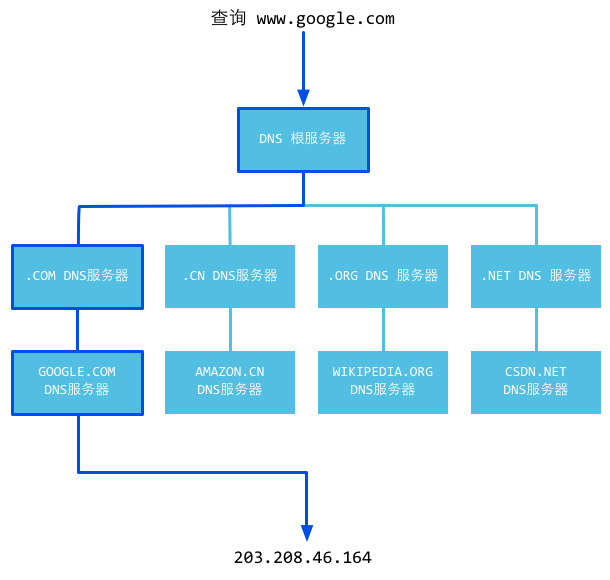
\includegraphics[width=14cm]{3.1.dns_hierachy.png}
   \label{図3.2}
   \caption{DNSの動作原理}
\end{figure}


より詳細なDNS解決のプロセスは下のようなものです。このプロセスは我々がDNSの作業モードを理解するのに助けとなります。

\begin{enumerate}
  \item ブラウザでwww.qq.comドメインを入力します。オペレーティングシステムはまず自分のローカルのhostsファイルにこのアドレスがないか検査します。もしあれば、このIPアドレスの設定が適用されます。ドメイン解決終了。
  \item もしhostsにこのドメインの設定がなければ、ローカルのDNSリゾルバのバッファを探します。もしあれば、これを返します。ドメイン解決終了。
  \item もしhostsとローカルのDNSリゾルバのバッファのどちらにも目的のドメインがなかった場合、まずTCP/IPのオプションで設定されているプライマリDNSサーバを探します。ここではこれをローカルDNSサーバと呼びましょう。このサーバが要求を受けた時、もし要求したドメイン名がローカルで設定されたリソースの中に含まれている場合、解決の結果をクライアントに返します。ドメイン解決終了。これは権威ある解決です。
  \item もし要求したドメイン名がローカルDNSサーバのゾーンでは解決できなかったものの、このサーバがこのURLをバッファリングしていた場合このIPアドレスが適用されます。ドメイン名解決終了。これは権威ある解決ではありません。
  \item もしローカルDNSサーバがそのゾーンファイルとバッファリングのどちらも有効でなかった場合、ローカルDNSサーバの設定に従って(リピータが設定されているか)検査を行います。もし転送モードが使用されていなければローカルDNSはリクエストを"ルートDNSサーバ"に送ります。"ルートDNSサーバ"はリクエストを受け取った後このドメイン名(.com)が誰によって権限を受け管理されているか判断し、このトップレベルドメインの権威サーバのIPを返します。ローカルDNSサーバがIP情報を受け取った後、.comドメインを担当するこのサーバと接続を行います。.comドメインを担当するサーバがリクエストを受け取った後、もし自分で名前解決できなければ、.comドメインを管理するもう一つ下のレイヤーのDNSサーバのアドレス(qq.com)をローカルDNSサーバに送ります。ローカルDNSサーバがこのアドレスを受け取った後、qq.comドメインのサーバを探し出し、www.qq.comのホストが見つかるまで上の動作を繰り返します。
  \item もし転送モードを使用していれば、このDNSサーバはリクエストをひとつ上のレイヤーのDNSサーバに転送します。このサーバが名前解決を行い、名前が解決できなかった場合は、ルートDNSを探すか、もう一つ上のレイヤーのにリクエストを転送します。またはルートが提示されます。最後に結果をローカルDNSサーバに返し、このDNSサーバはクライアントに返します。
\end{enumerate}


\begin{figure}[H]
  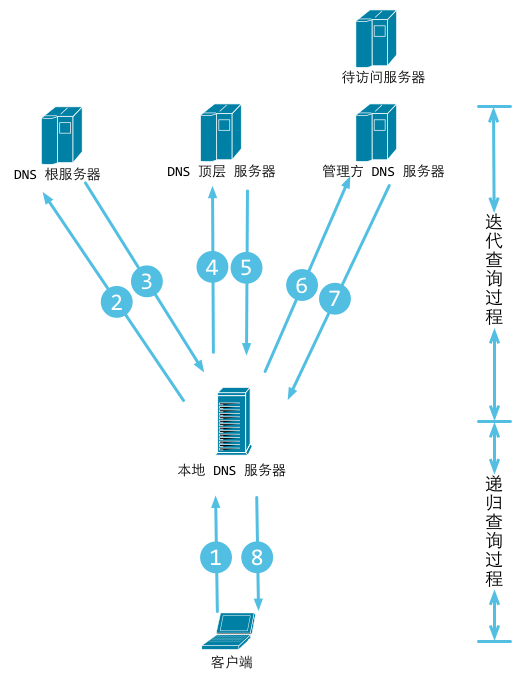
\includegraphics[width=14cm]{3.1.dns_inquery.png}
   \label{図3.3}
   \caption{DNS解決の全体のプロセス}
\end{figure}


\begin{quote}
いわゆる再帰検索プロセスは"検索者"の交代を意味します。また、反復する検索プロセスでは"検索者"は不変です。

例をあげて説明しましょう。あなたは一緒に法律の授業を受けている女の子の電話番号を知りたいとします。あなたはこっそり彼女の写真も撮っています。寝室にもどって、正義感の強いアニキたちにそのことを伝えます。このアニキたちは異議を唱えることもなく、胸を叩いてあなたにこう言います。「急ぐ必要はない。私があなたに替わって調べてあげましょう」(この時一時再帰検索が完了しています。すなわち、検索者の役割が変更されました。)。その後彼は写真を携え学部の4年生の先輩のところに聞きにいきます。「この女の子はxx学部なんですけど・・・」その後このアニキは矢継ぎ早にxx学部のオフィス主任の助手を務めているクラスメートに聞きます。このクラスメートはxx学部のyyゼミであると言います。またこの正義感の強いアニキたちはxx学部のyyゼミのゼミ長のところにいき、この女の子の電話番号をゲットします。(ここまでで何回かの連続検索が完了しました。すなわち、検索者の役は変わっていませんが、聞きに行く対象を反復して取り替えています。)最後に彼は番号をあなたの手に渡すことで全体の検索が完了します。
\end{quote}

上のステップを通して、IPアドレスを最後に取得します。つまりブラウザが最後にリクエストを送る時はIPにもとづいて、サーバと情報のやりとりをするのです。


